
\let\textcircled=\pgftextcircled
\chapter{The Compute Unit}

\label{chap:compute_unit}

\section{Overview}
\paragraph{}

This chapter discusses the various Boolean and arithmetic operations that we have implemented in our memory architecture. The working of these operations is also explained in detail with their corresponding simulation outcomes for each case.

\section{NAND , NOR and COMPLEMENT}
\paragraph{}

For NAND/NOR operation the RBL is precharged to Vdd. The precharged RBL will eventually go to 0V if Q for any 1 of the input operand is ‘1’.However, the fall time of the signal at RBL from the precharged value to 0V would depend strongly on whether any one Q is high or if both the Q bits are high simultaneously. If both the Qs are ‘1’, the discharge rate of the precharged RBL line would be twice of that when only 1 of the Q is '1'.We Use this property of different rate of discharging to our advantage.

\begin{figure}[h]
 
\begin{subfigure}{0.5\textwidth}
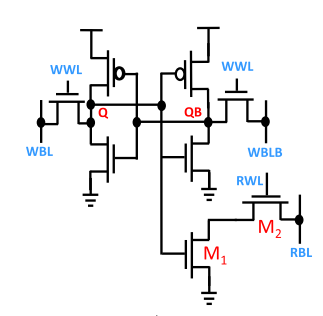
\includegraphics[width=0.9\linewidth, height=5cm]{1.PNG} 
\caption{ Schematic of a standard 8T-SRAM bit-cell}
\label{fig:subim1}
\end{subfigure}
\begin{subfigure}{0.5\textwidth}
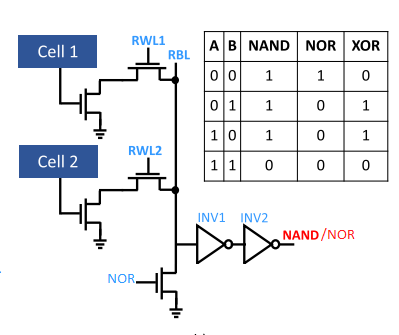
\includegraphics[width=0.9\linewidth, height=5cm]{2.PNG}
\caption{Single ended sensing of NAND/NOR.(Truth table for NAND/NOR/XOR included)}
\label{fig:subim2}
\end{subfigure}
 
\caption{Basic schematic for Nand and Nor operation[2]}
\label{fig:image1}
\end{figure}

In order to exploit the different discharge rates of the RBL lines, the RWL signal had to be timed such that the RBL does not discharge completely in cases of ‘01/10’. This allows a significant difference in voltage levels on RBL in the two cases (‘01/10’ and ‘11’). The switching threshold of INV1 is  chosen such that it will go high only for
the case when both bits are '1’.thus output of inverter INV2 will mimic the NAND operation.

For NOR operation will use an extra discharge transistor, which will discharge the RBL for 1 time period. Thus even in the case of ('01/10'), RBL voltage will reach level same as that of '11', and for '11' case the RBL voltage will fall to even lower value, thus for all 3 cases '01/10/11' the RBL goes below the switching threshold of INV1. Thus it will exhibit NOR operation.

For NOT operation of a single variable, we can use NOR operation itself.As NOR of any signal with '0' will give complement of the signal itself.

A NOR B = (A + B)' = A'.B'

If Only 1 RWL is activated then it is equivalent to one element being '0'. 

Thus A'.1=A' 

\begin{figure}[h]
 \centering
\begin{subfigure}{0.4\textwidth}
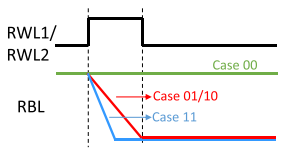
\includegraphics[width=\linewidth, height=4cm]{3.PNG} 
\caption{NOR output for cell 1 and cell 2}
\label{fig:subim1}
\end{subfigure}
\begin{subfigure}{0.4\textwidth}
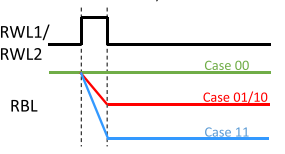
\includegraphics[width=\linewidth, height=4cm]{4.PNG}
\caption{NAND output for cell 1 and cell 2}
\label{fig:subim2}
\end{subfigure}
 
\caption{Timing diagrams for NAND and NOR[2]}
\label{fig:image2}
\end{figure}


For simulation purposes we assume our bit line capacitance = 10f F. 

The inverter in our case is biased such that its switching threshold = 0.7V.

We have our pulse width =75 ps

Average voltage drop from a single bit in one pulse is 0.6V.

\begin{figure}[h]
    \centering
    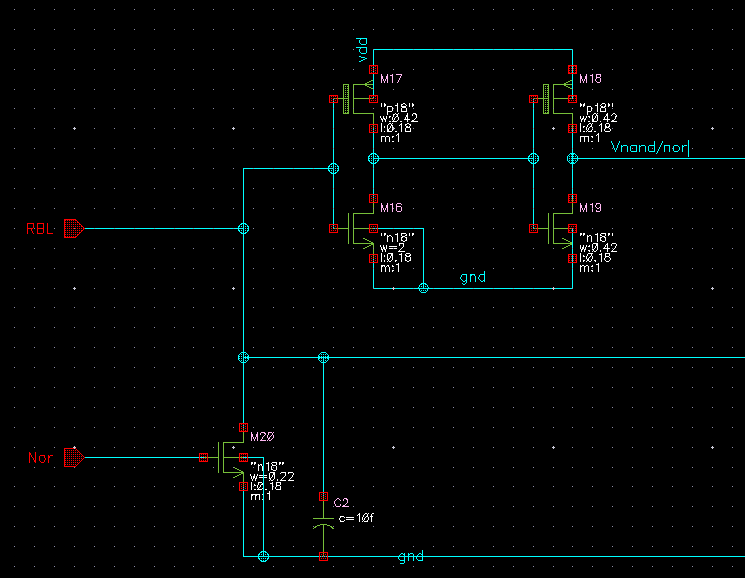
\includegraphics[width=0.6\textwidth]{nand_nor.png}
    \caption{NAND/ NOR detection circuit with sizing}
    \label{fig:mesh1}
\end{figure}
`
\begin{figure}[H]
\begin{center}
\begin{subfigure}{0.4\textwidth}
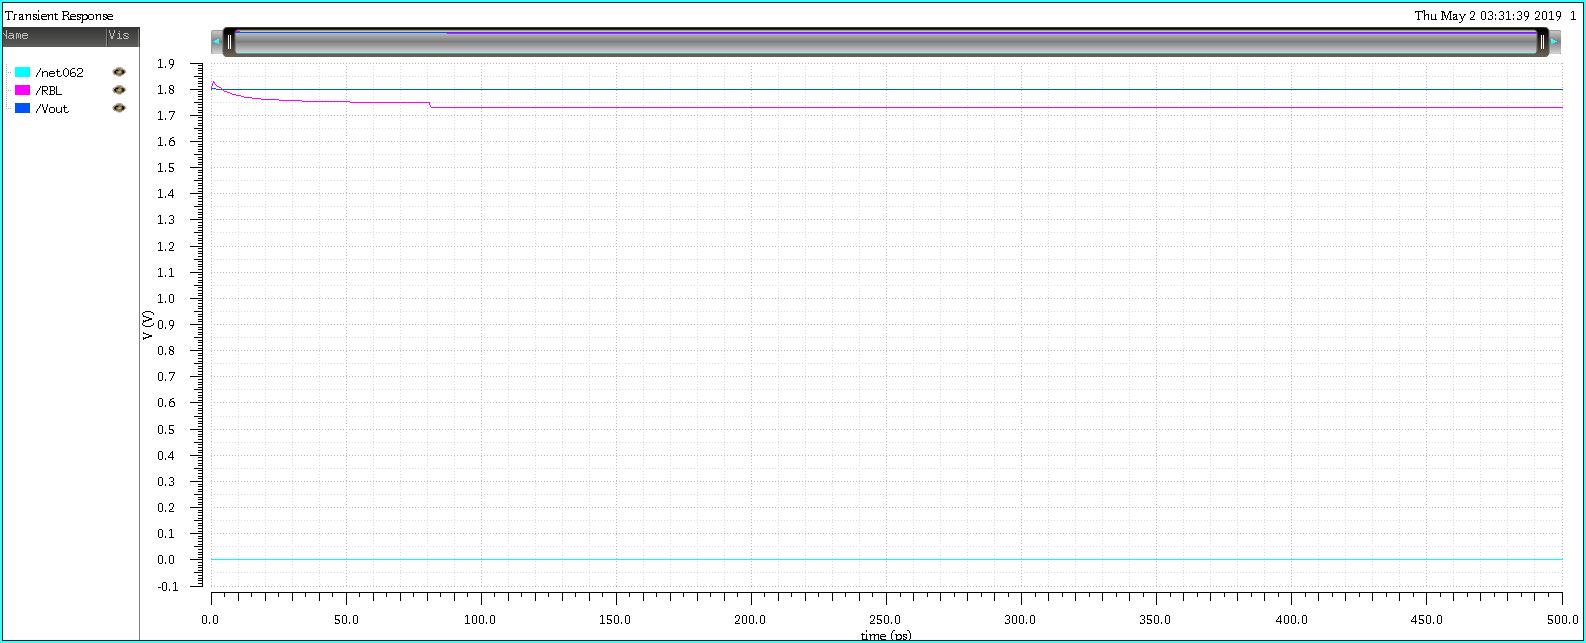
\includegraphics[width=\textwidth]{nand00.png}
\caption{00}
\end{subfigure}
\begin{subfigure}{0.4\textwidth}
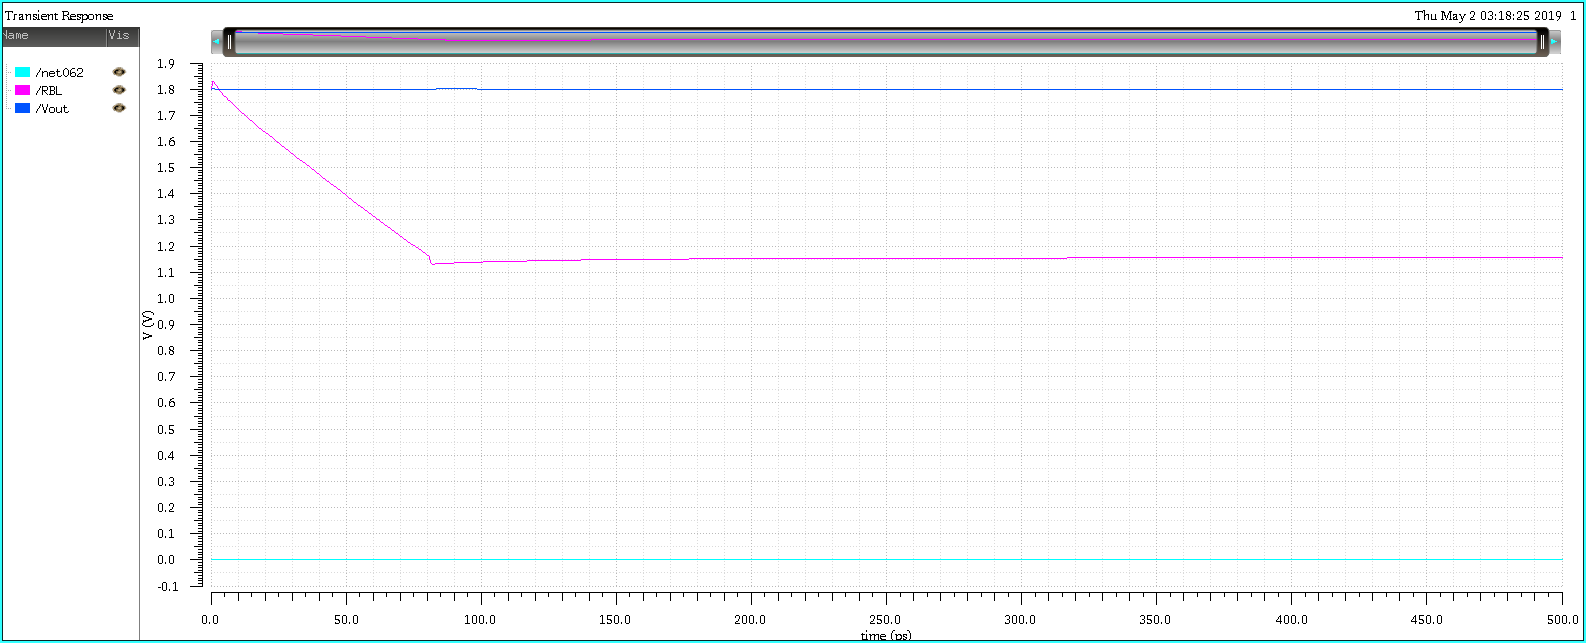
\includegraphics[width=\textwidth]{nand01.png}
\caption{01}
\end{subfigure}
\begin{subfigure}{0.4\textwidth}
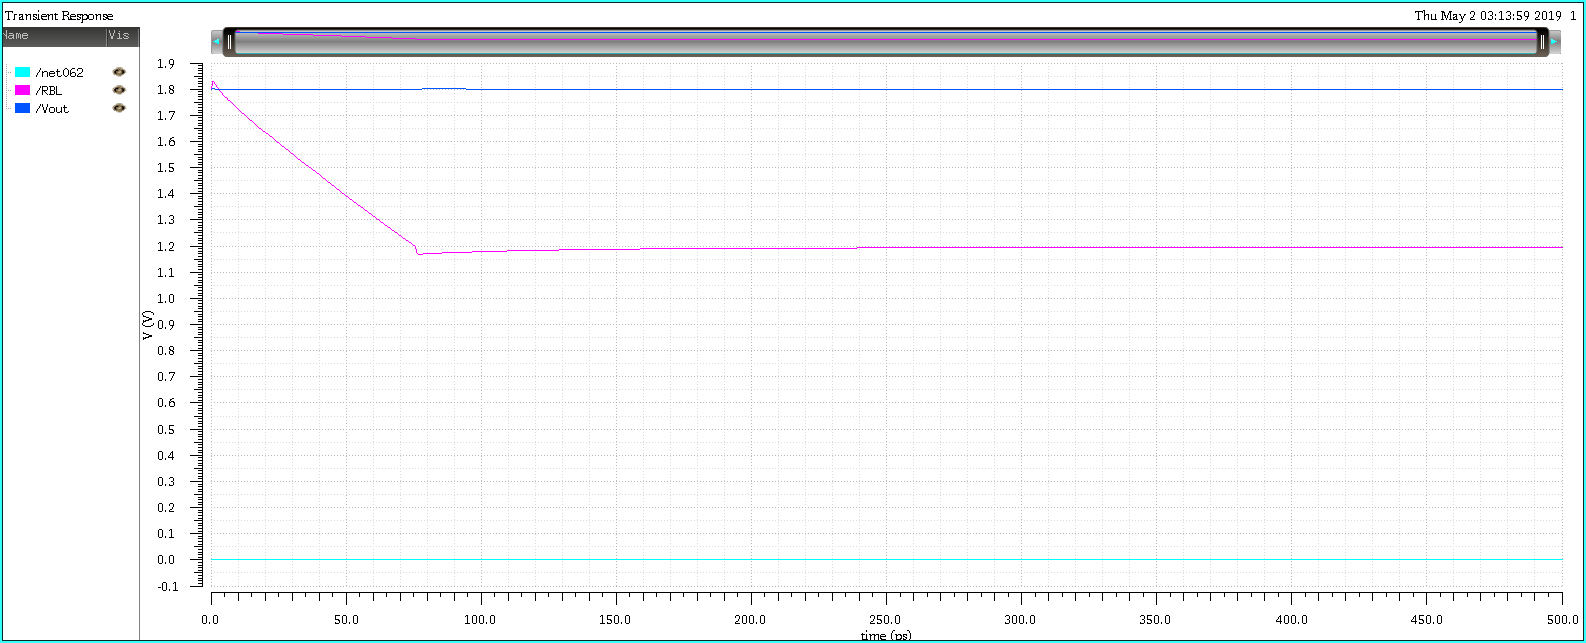
\includegraphics[width=\textwidth]{NAND10.png}
\caption{10}
\end{subfigure}
\begin{subfigure}{0.4\textwidth}
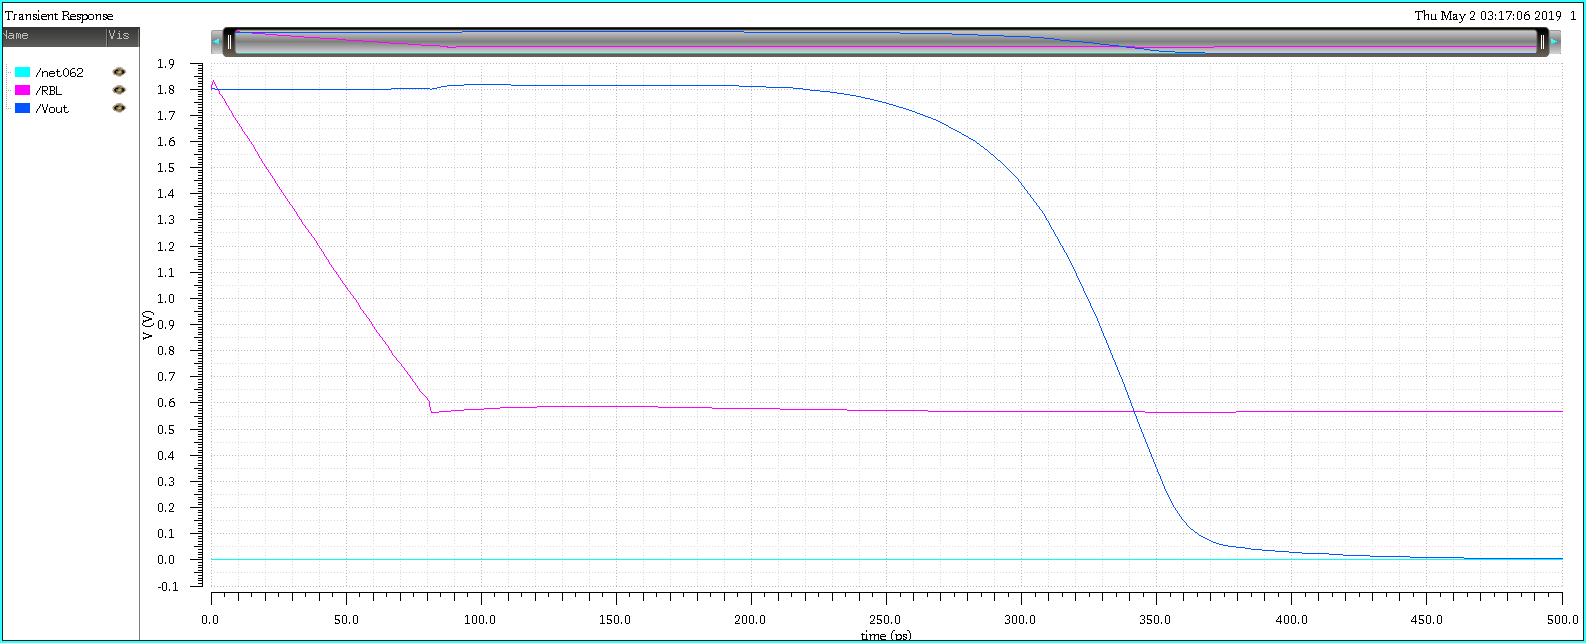
\includegraphics[width=\textwidth]{nand11.png}
\caption{11}
\end{subfigure}
\end{center}
\caption{Simulation output for NAND }

\end{figure}

\begin{figure}[H]
\begin{center}
\begin{subfigure}{0.4\textwidth}
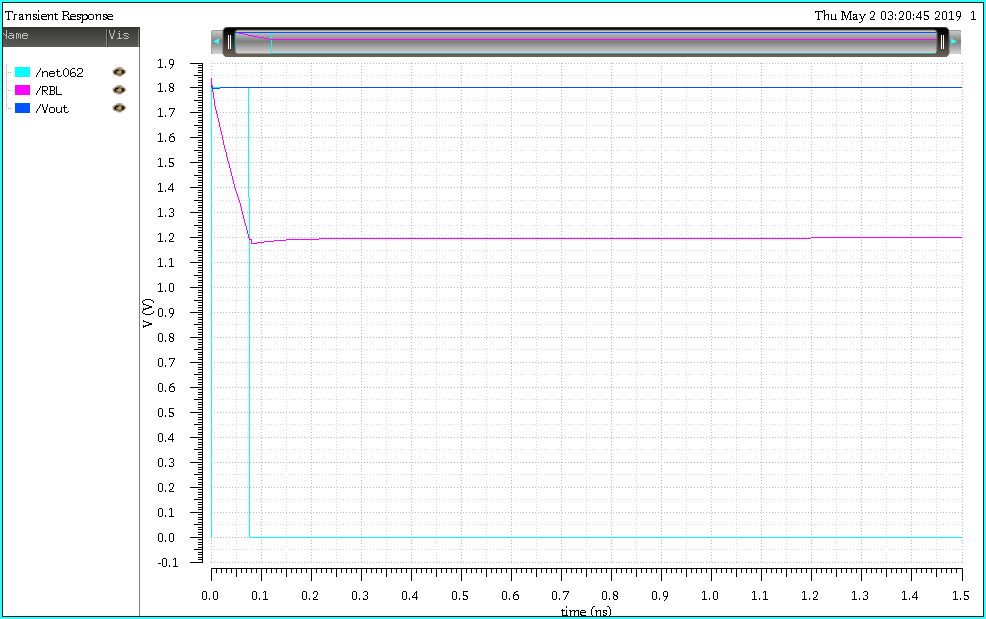
\includegraphics[width=\textwidth]{nor00.png}
\caption{00}
\end{subfigure}
\begin{subfigure}{0.4\textwidth}
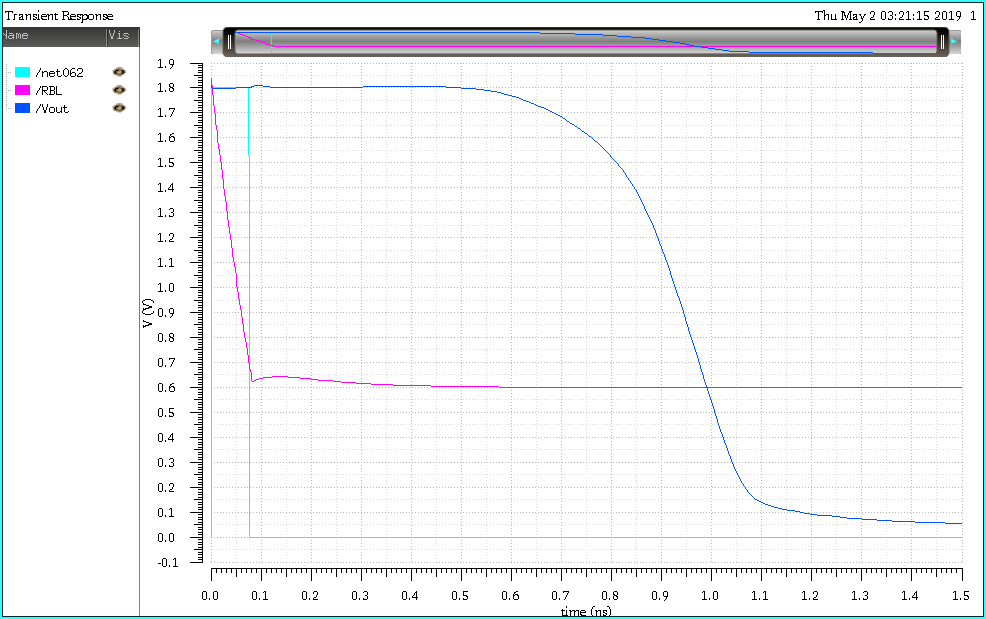
\includegraphics[width=\textwidth]{nor01.png}
\caption{01}
\end{subfigure}
\begin{subfigure}{0.4\textwidth}
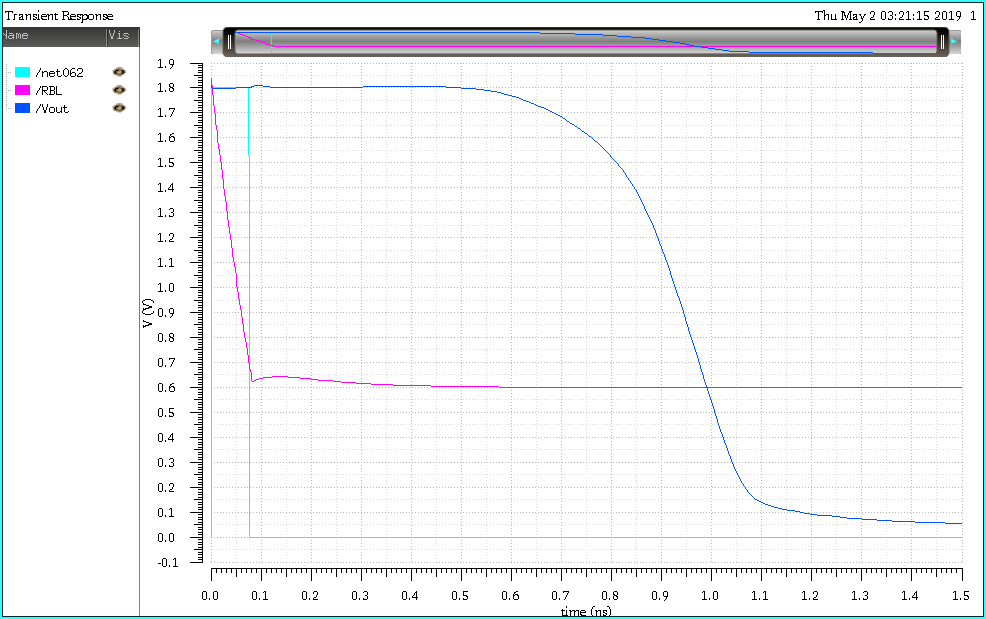
\includegraphics[width=\textwidth]{nor10.png}
\caption{10}
\end{subfigure}
\begin{subfigure}{0.4\textwidth}
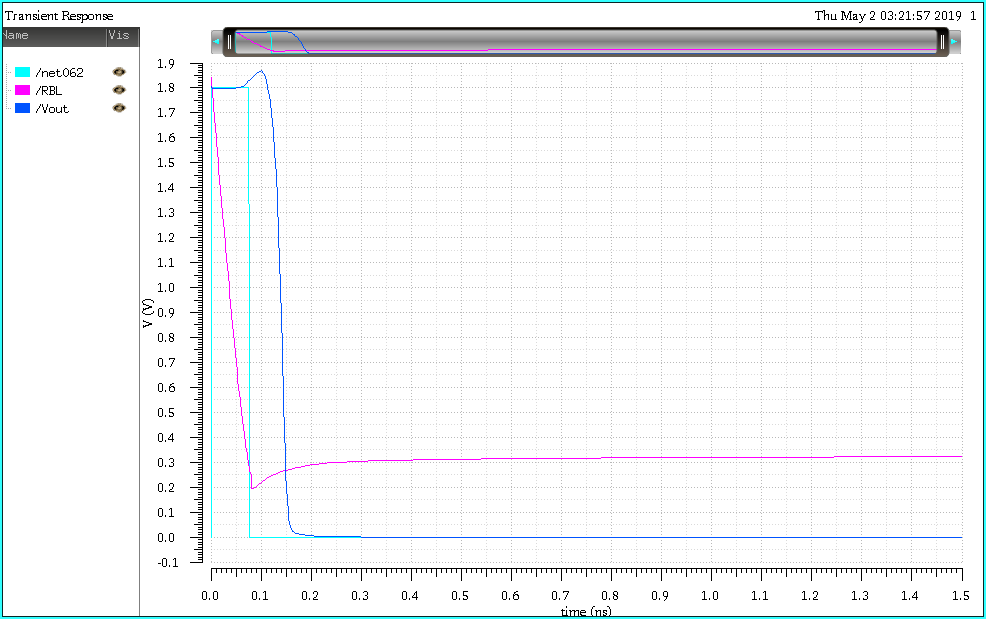
\includegraphics[width=\textwidth]{nor11.png}
\caption{11}
\end{subfigure}
\end{center}
\caption{Simulation output for NOR }

\end{figure}


\section{XOR}
\paragraph{}

XOR operation(Exclusive OR) gives 1 when either of the input is 1.As we have seen in the last section.

Pulse Width,$$\tau = 75ps$$

Thus voltage drop from single '1' =0.6V.(For C=10f F)

Thus, we need to find a circuit which detects the intermediate voltage but give 0 for either low (V<0.8) or high (V >1.4) voltage range.

\begin{figure}[h]
    \centering
    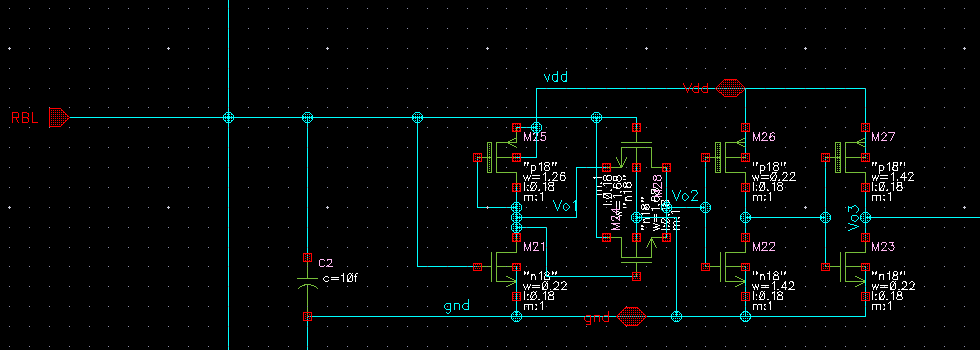
\includegraphics[width=0.7\textwidth]{zor.png}
    \caption{XOR detection circuit with sizing}
    \label{fig:mesh1}
\end{figure}

The XOR detection circuit consists of 3 parts.

\begin{itemize}
    \item The First part is a linear inverter, which gives Vl = Vdd-Vin( nearly equal).
    \item The next part consist of 2 NMOS, whose drain and gate are inter-connected.That is Gate of M3 and drain of M4 is Vin.The Gate of M4 and drain of M3 is Vp. The source of both MOSFET are joined together. 
    \item The final part is a buffer to ensure rail to rail swing at the output of the circuit.
\end{itemize}

Thus combining all 3 parts gives a circuit which detects intermediate voltage levels. Figure 4.7 show the DC response of circuit. The response is for a given particular biasing and can be shifted to either right or left according to needs by changing the biasing of the circuit. 

\begin{figure}[h]
    \centering
    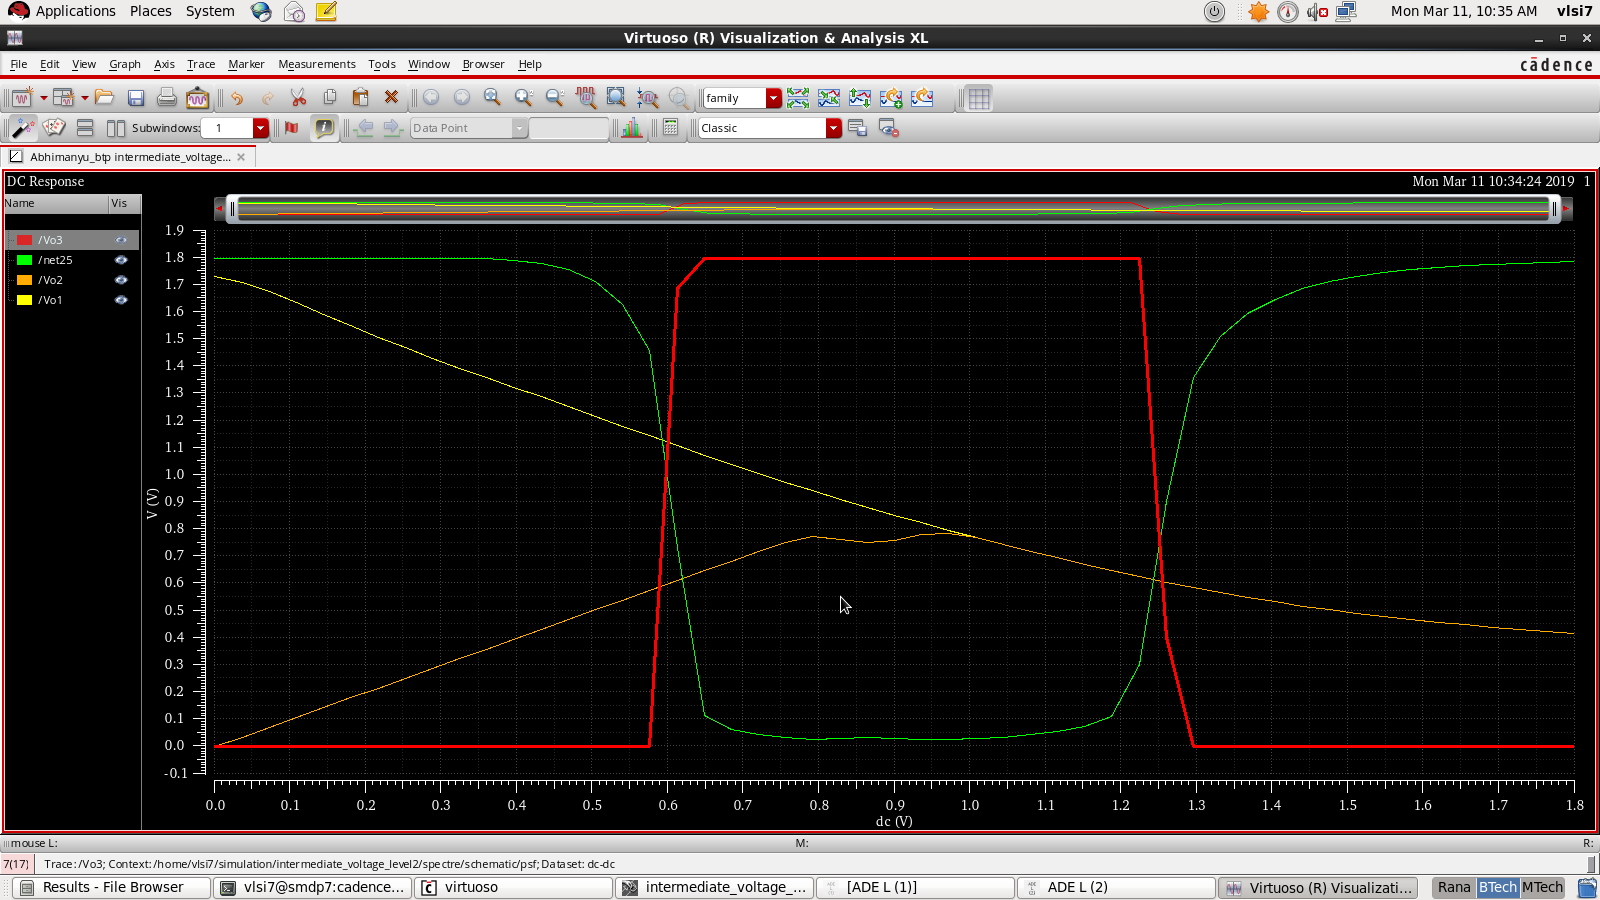
\includegraphics[width=0.6\textwidth]{xor_dc.png}
    \caption{XOR circuit DC response}
    \label{fig:mesh1}
\end{figure}

The figure 4.8 shows the output of the simulation of the XOR circuit for RBL for 2 bit column.
\begin{figure}[H]
\begin{center}
\begin{subfigure}{0.4\textwidth}
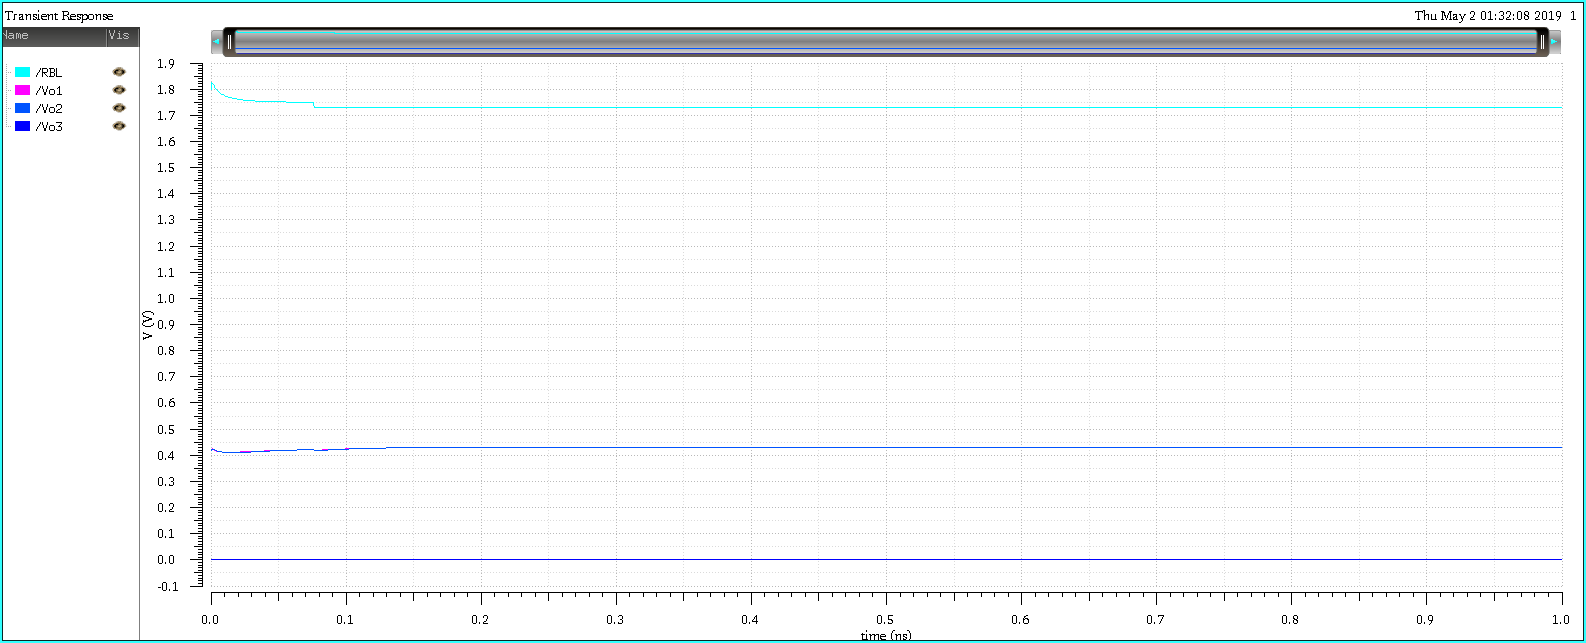
\includegraphics[width=\textwidth]{xor00.png}
\caption{00}
\end{subfigure}
\begin{subfigure}{0.4\textwidth}
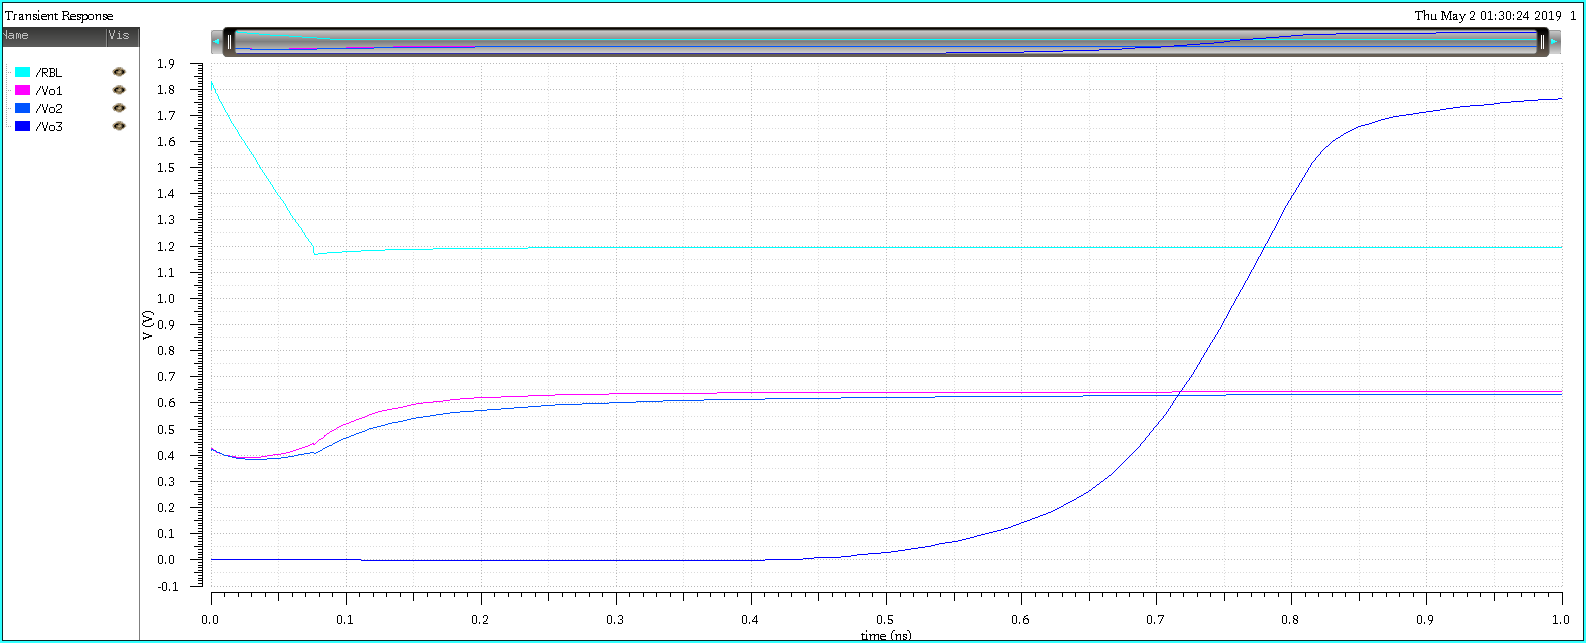
\includegraphics[width=\textwidth]{xor01.png}
\caption{01}
\end{subfigure}
\begin{subfigure}{0.4\textwidth}
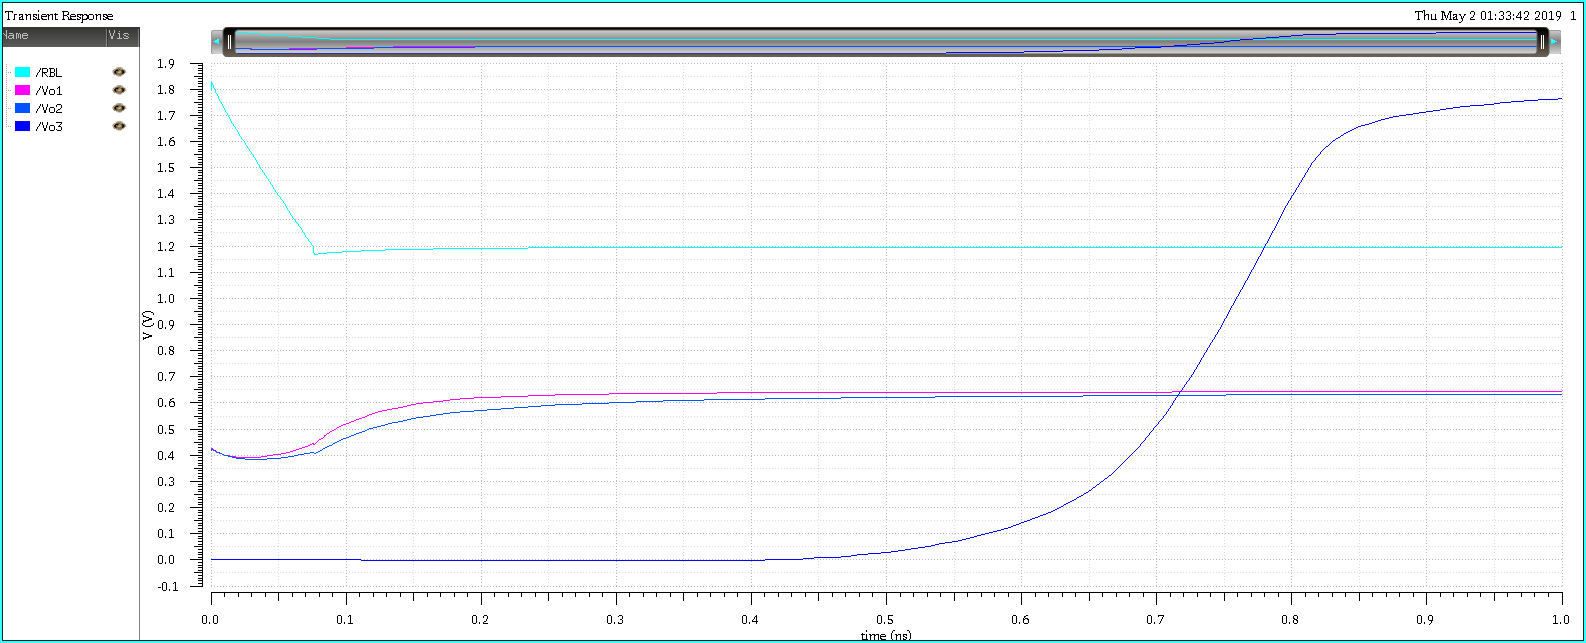
\includegraphics[width=\textwidth]{xor10.png}
\caption{10}
\end{subfigure}
\begin{subfigure}{0.4\textwidth}
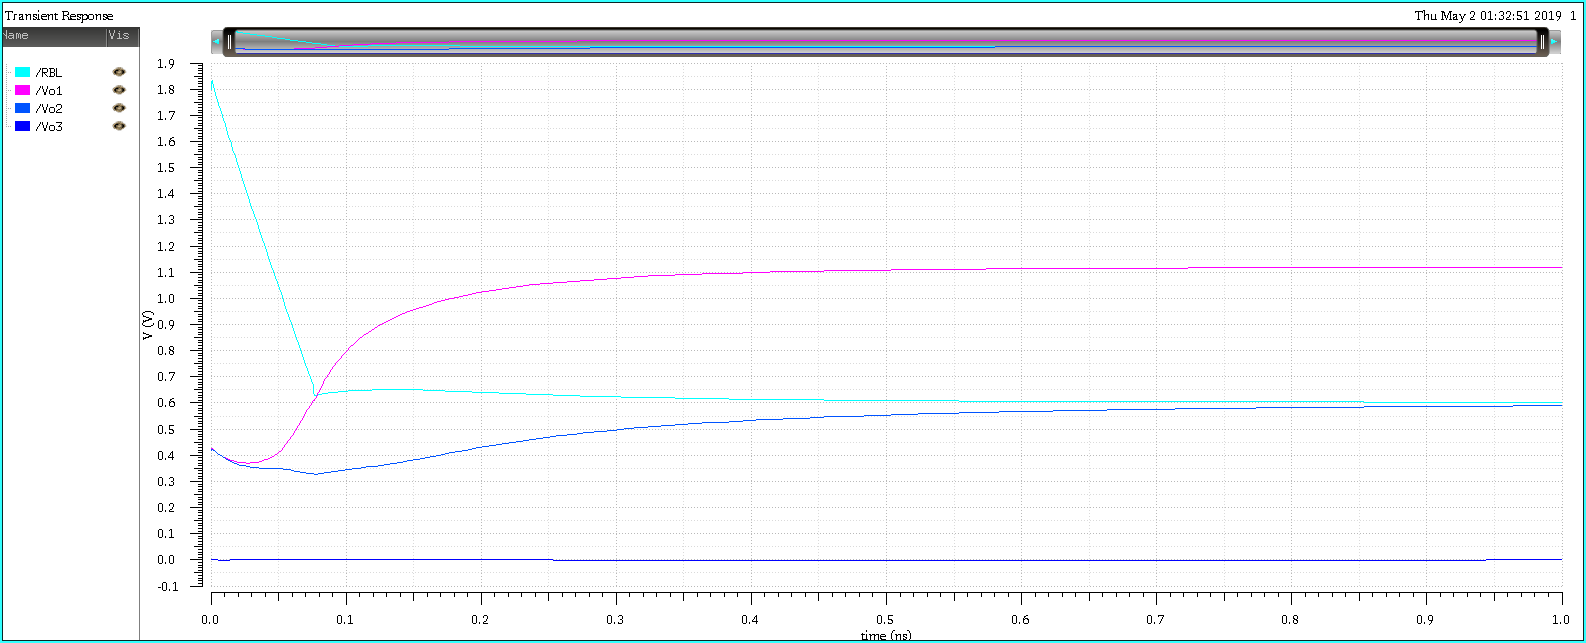
\includegraphics[width=\textwidth]{xor11.png}
\caption{11}
\end{subfigure}
\end{center}
\caption{Simulation output for XOR }

\end{figure}


\section{ADDITION \& SUBTRACTION}
\paragraph{}

Addition operation is one of the most basic arithmetic operation, and is almost needed in all types of uses.We are here performing 4 bit addition(As word each word is of 4 bits). For a simple Boolean addition each pair create a SUM and a Carry.

    An + Bn = \{Cn,Sn\}
    
    \{A3,A2,A1,A0\} + \{B3,B2,B1,B0\}  = \{C3,S3,S2,S1,S0\} 

For Half adder

Sn = An $\bigotimes$ Bn  (An XOR Bn)

Cn = An.Bn   (An AND Bn)

For Full adder

Sn = An $\bigotimes$ Bn $\bigotimes$ Cn-1

Cn = An.Bn + Cin.(An $\bigotimes$ Bn)

As for all the bits in the word the (An $\bigotimes$  Bn) ,will be computed simultaneously.But the Carry would have to propagate from first to last digit.This will become the deciding factor or the bottleneck. As it is clear from above equations , we get our half adder output from previously computed operation, that is XOR and NAND.

S = Cin  $\bigotimes$ (An $\bigotimes$ Bn)

Cout = (((An $\bigotimes$ Bn).Cin)'.(A.B)')'

So for computing XOR and NAND with Cin, we need standard logic gates.Schematic of these gates with shown in figure 4.10 

\begin{figure}[h]
    \centering
    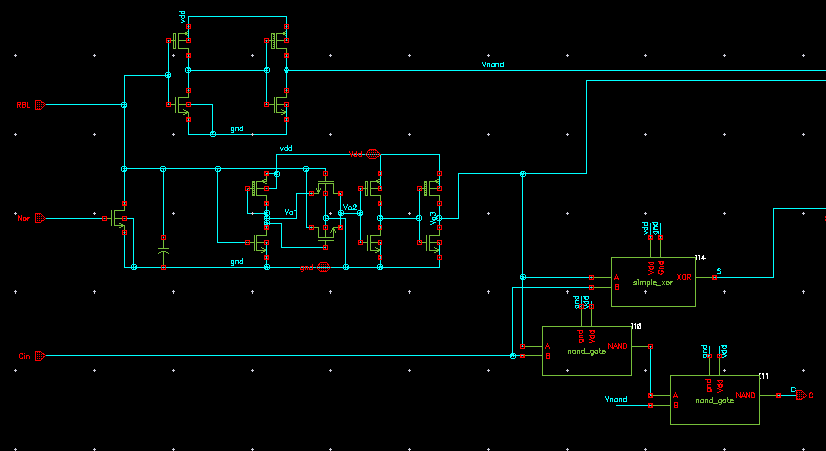
\includegraphics[width=0.7\textwidth]{add.png}
    \caption{Add circuit using results from XOR and NAND}
    \label{fig:mesh1}
\end{figure}

\begin{figure}[h]
\begin{center}
\begin{subfigure}{0.4\textwidth}
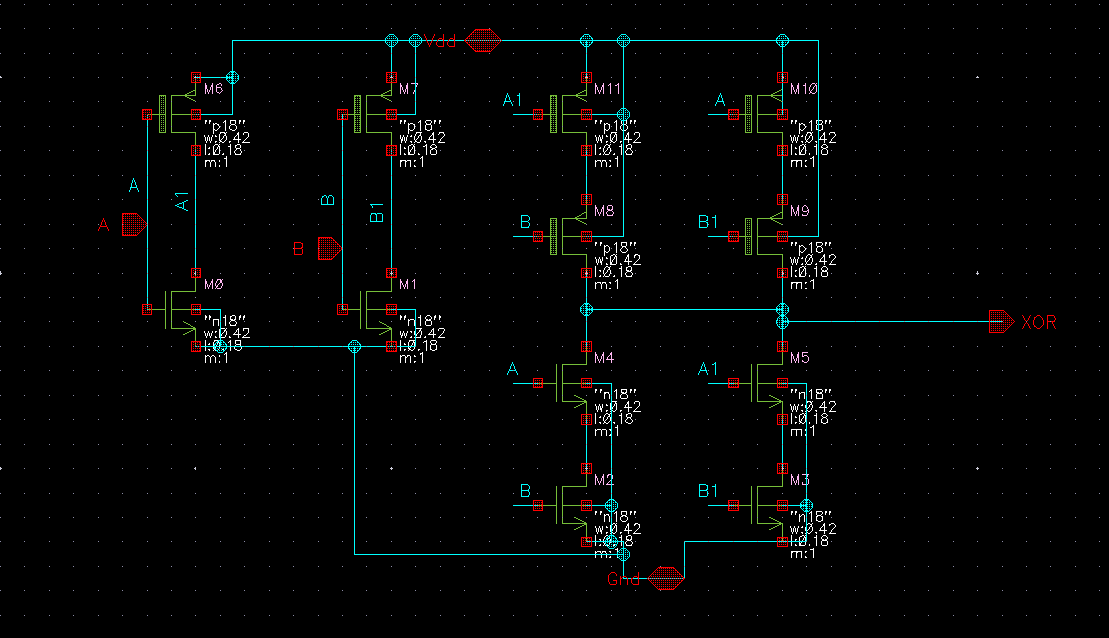
\includegraphics[width=\textwidth]{chapters/chapter04/simple_xor_gate.png}
\caption{ XOR }
\end{subfigure}
\begin{subfigure}{0.4\textwidth}
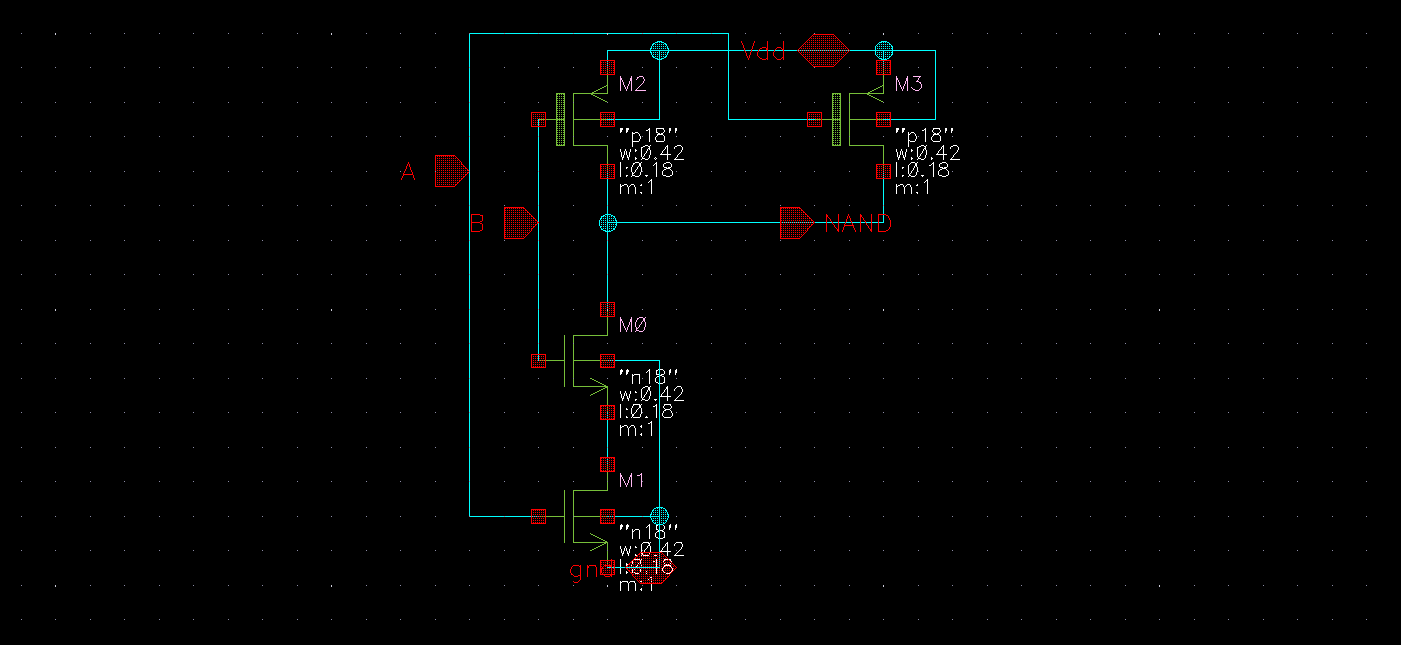
\includegraphics[width=\textwidth]{chapters/chapter04/nand_gate.png}
\caption{ NAND }
\end{subfigure}
\end{center}
\caption{Schematic of XOR and NAND gate }

\end{figure}


\begin{figure}[H]
\begin{center}
\begin{subfigure}{0.4\textwidth}
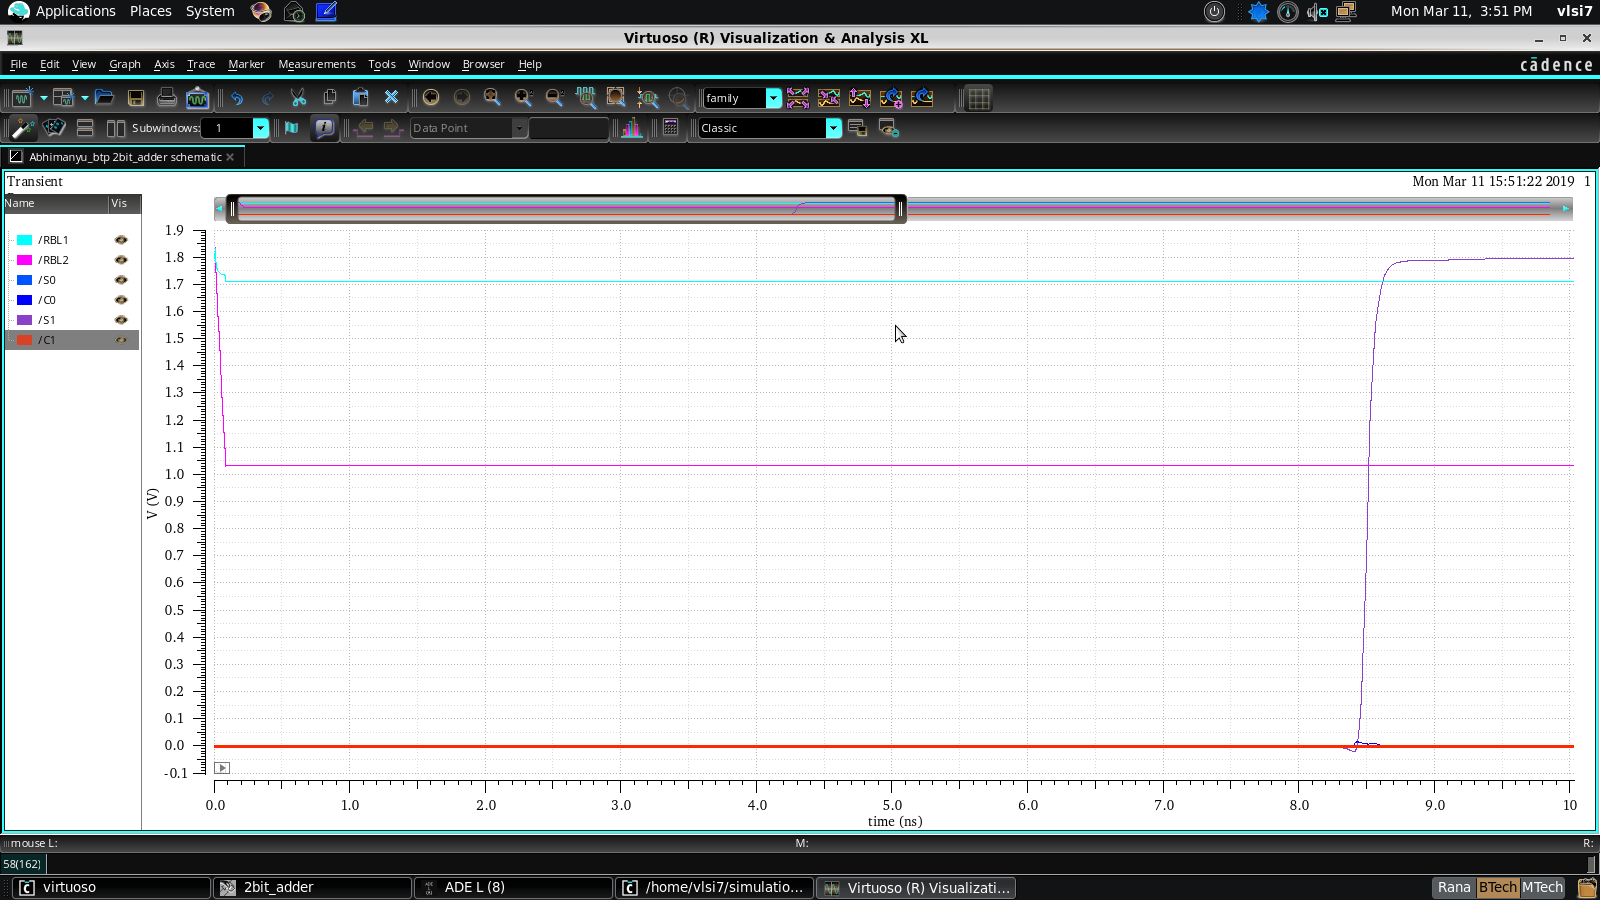
\includegraphics[width=\textwidth]{chapters/chapter04/add_00+10.png}
\caption{ 00 + 10 }
\end{subfigure}
\begin{subfigure}{0.4\textwidth}
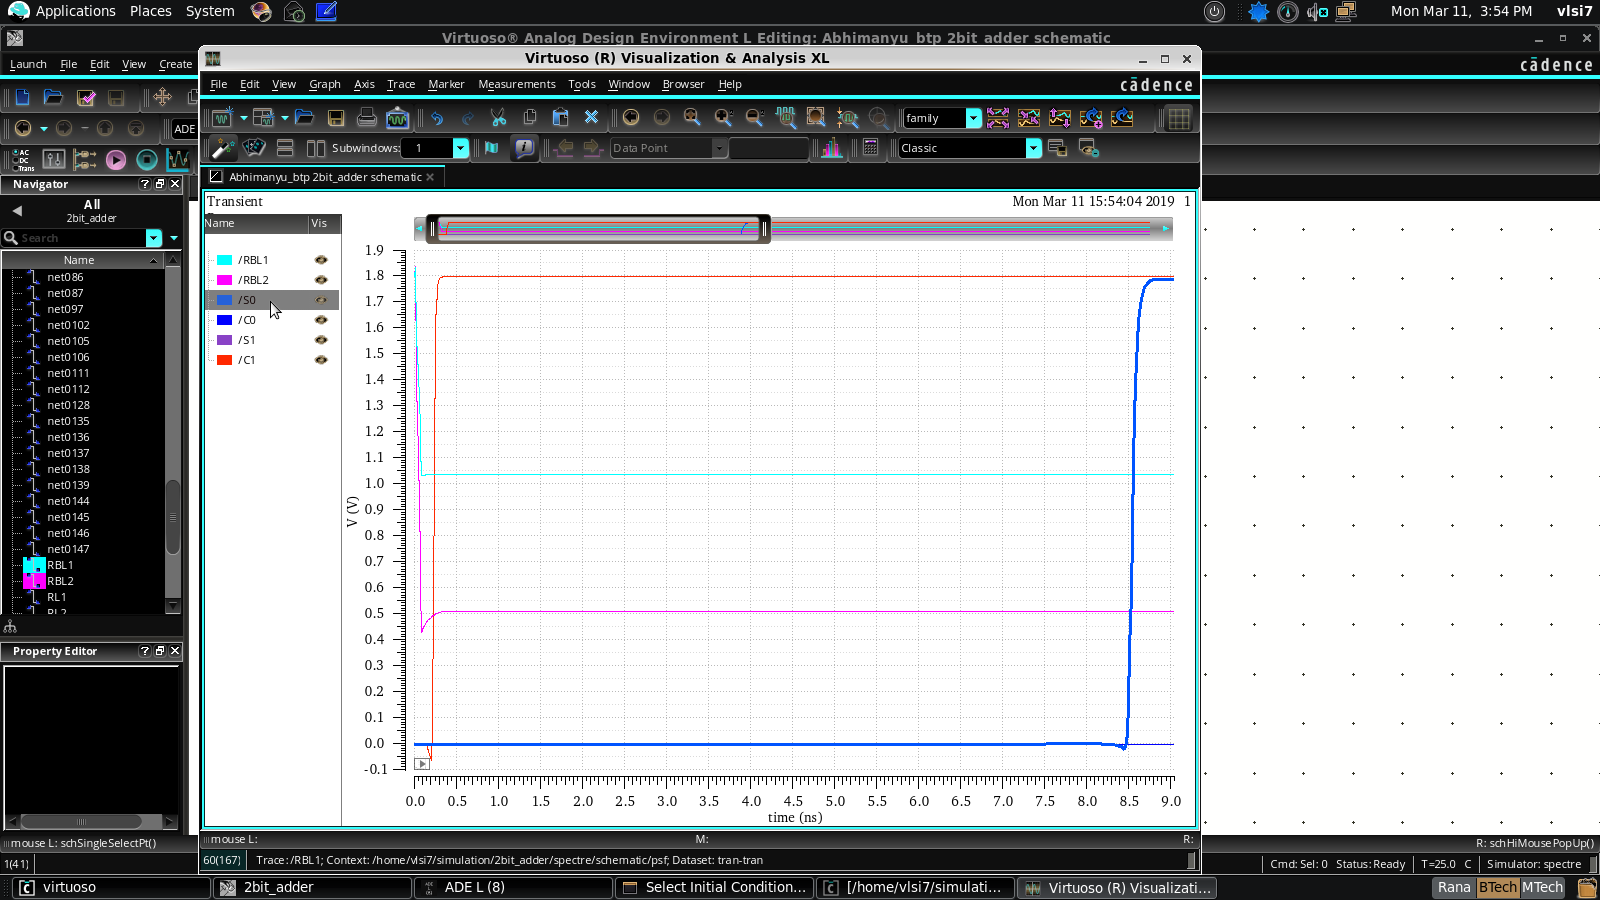
\includegraphics[width=\textwidth]{chapters/chapter04/add_11+10.png}
\caption{ 11 + 10 }
\end{subfigure}
\begin{subfigure}{0.4\textwidth}
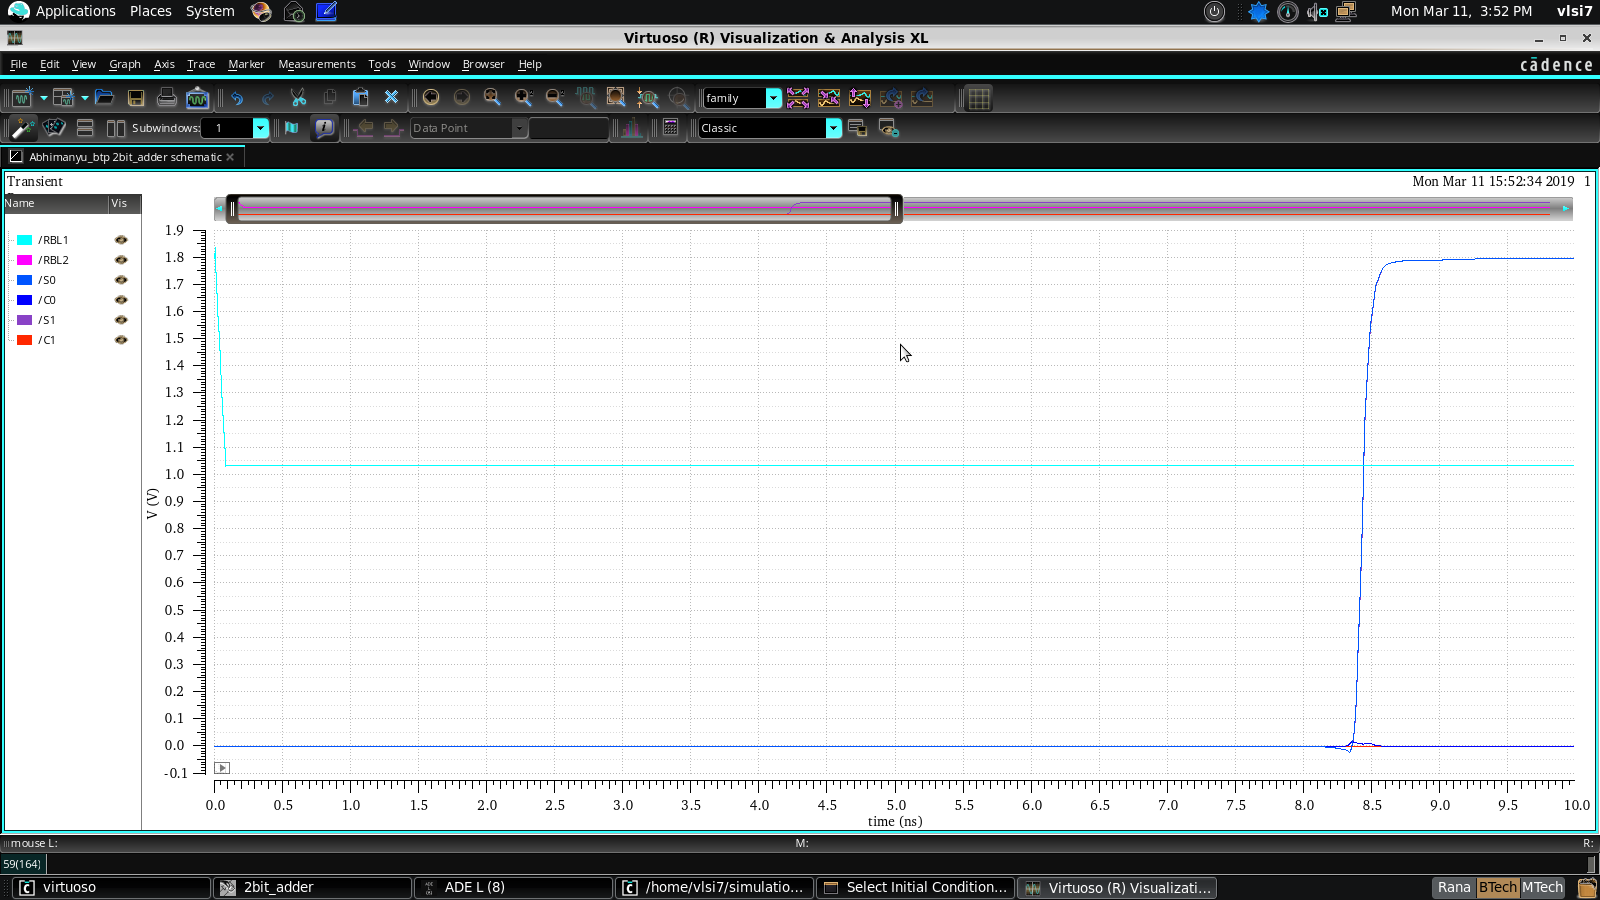
\includegraphics[width=\textwidth]{chapters/chapter04/add_10+01.png}
\caption{ 10 + 01 }
\end{subfigure}
\begin{subfigure}{0.4\textwidth}
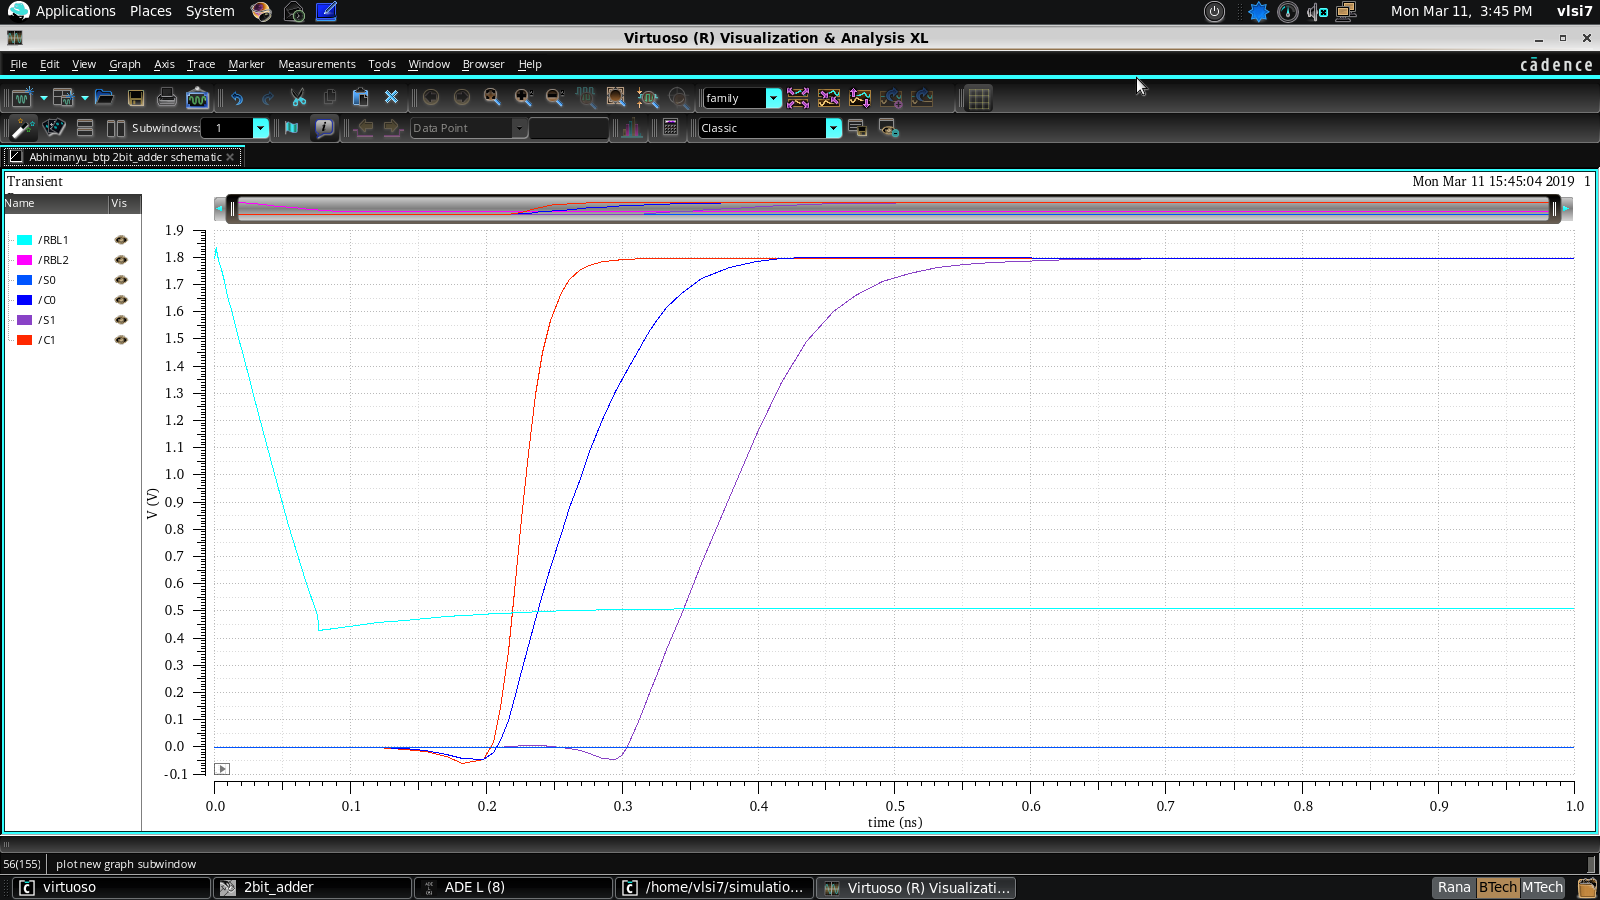
\includegraphics[width=\textwidth]{chapters/chapter04/add_11+11.png}
\caption{ 11 + 11 }
\end{subfigure}
\end{center}
\caption{Simulation output for ADD }

\end{figure}
\section{SHIFT}
\paragraph{}

The Shift operation enables to shift right and left by 1 Bit for a 4 bit word. As the size of the SRAM cell is small, we cannot use D Flip Flops to make a shift register here as there will be pitch mismatch along with unnecessary area consumption. To tackle this problem of shifting without Flip Flops, we have used 3T DRAM cells.

\begin{figure}[H]
\centering
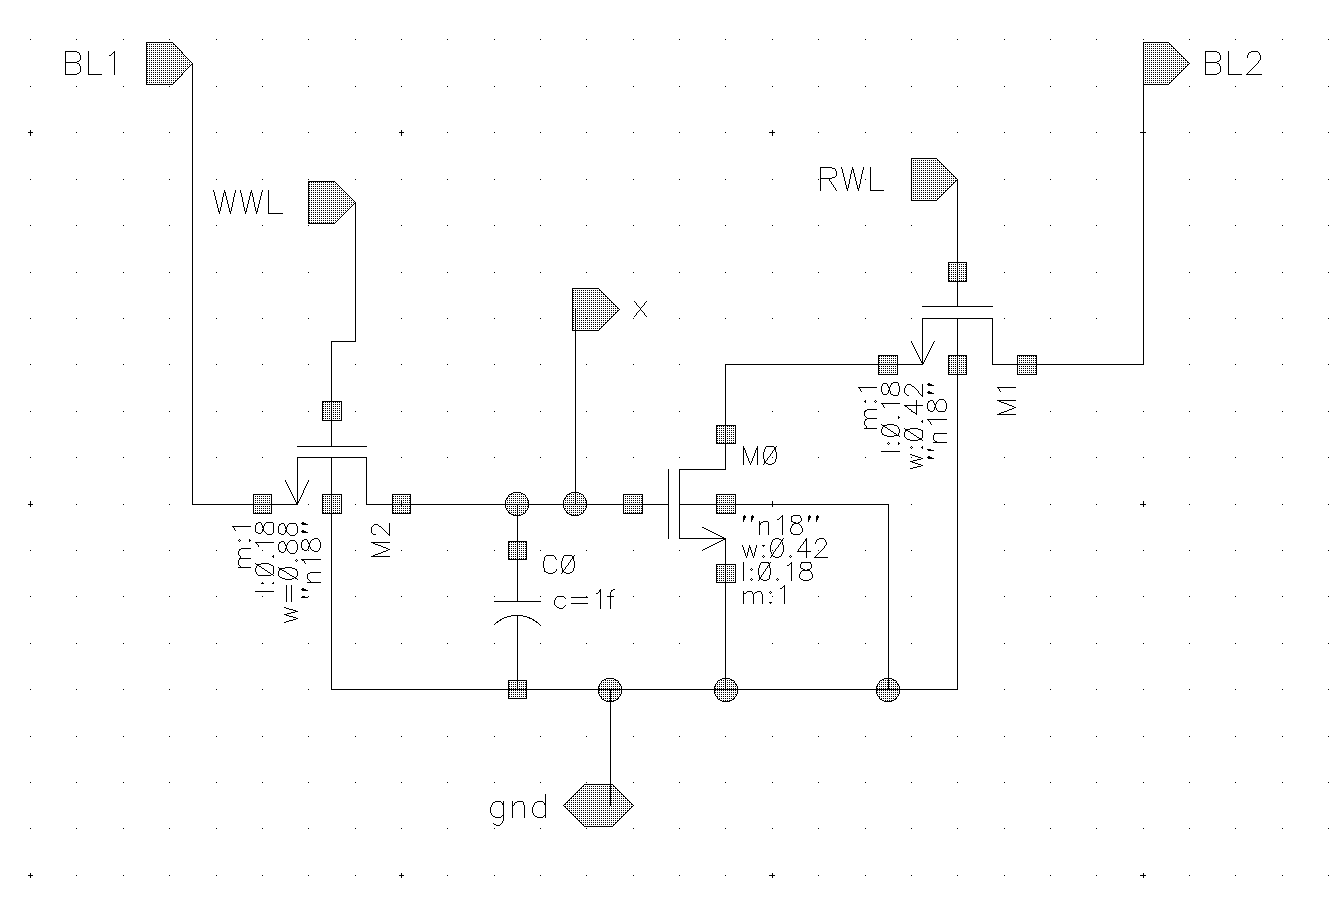
\includegraphics[width=0.5\textwidth]{dram1.png}
\caption{The 3T DRAM cell}
\label{fig:Figure}
\end{figure}

3T DRAM cell has a capacitor (1f F) to hold the bit value. The write operation is destructive but the read operation does not effect the stored value, and the complement of the stored value is given as output by the DRAM cell on read.

So we first copy the word into the DRAMs just below the SRAM word in the compute block, and then shift left or right among the DRAM cells. When the data is read from DRAM complement of the data stored is read. In a 1 bit shift a DRAM is read twice, first when it is read so that it can shift it's value to the nearest bit, then second time when it has to return back the shifted value to the SRAM cell. So by this way in a 1 bit shift the data finally stored in the SRAM is correct and not the complement.

\begin{figure}[H]
\centering
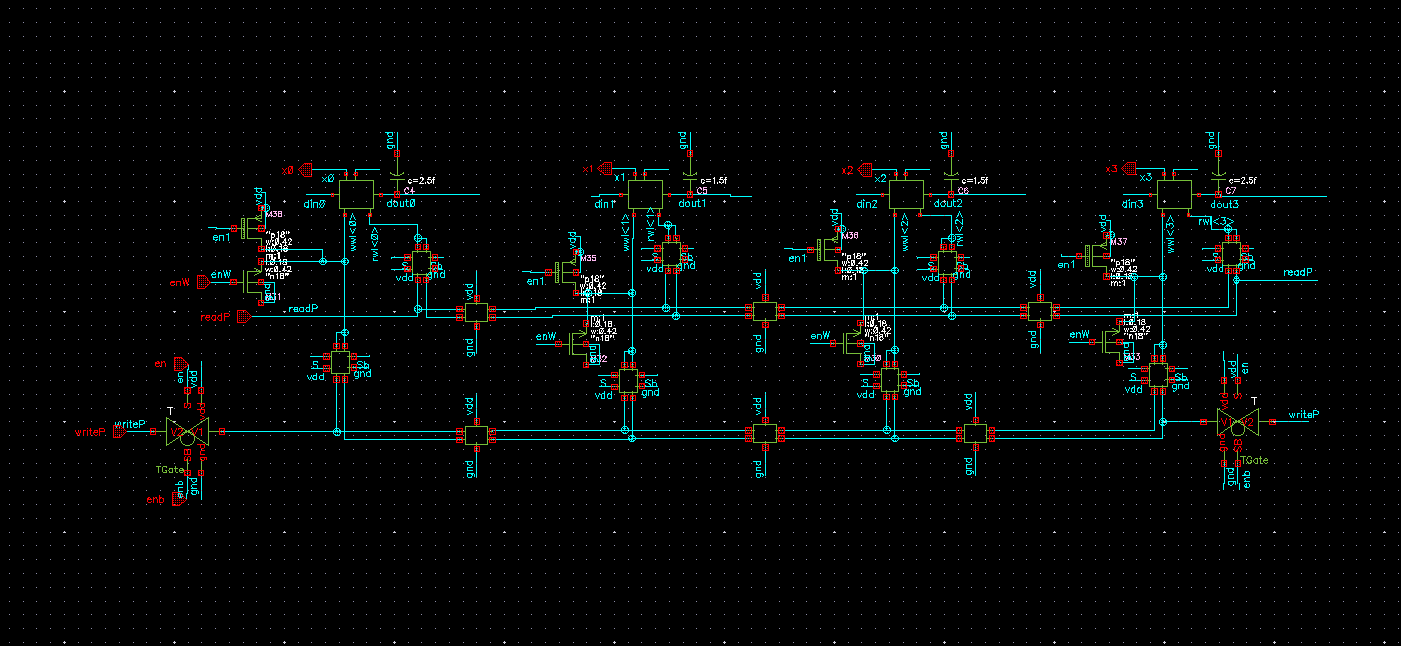
\includegraphics[width=0.7\textwidth]{shift_blk.png}
\caption{The DRAM shifter design}
\label{fig:Figure}
\end{figure}

So, the data is shifted sequentially starting form the MSB if we are shifting left and LSB if we are shifting right to avoid the loss of data. In a 4 bit word, for a left shift first the MSB or 4th bit is written by the 3rd bit, then 3rd is written by 2nd, 2nd by 1st bit and the 1st bit or LSB is set to 1. So, analysing this situation we see that the MSB is first written and sequentially the write signal is moving towards the LSB along with the read signal from the previous bit. 

Therefore, a single write and read pulse from the left can be sent towards the LSB with finite delay in between the DRAM's Write and Read enable to give time to shift 1 bit. Similar technique can be used for the right shift. The delay element placed between two DRAMs consists of a chain of inverters. MUX is used to select if the circuit is going to left shift or right shift according to the control signal.

\begin{figure}[H]
\begin{center}
\begin{subfigure}{0.7\textwidth}
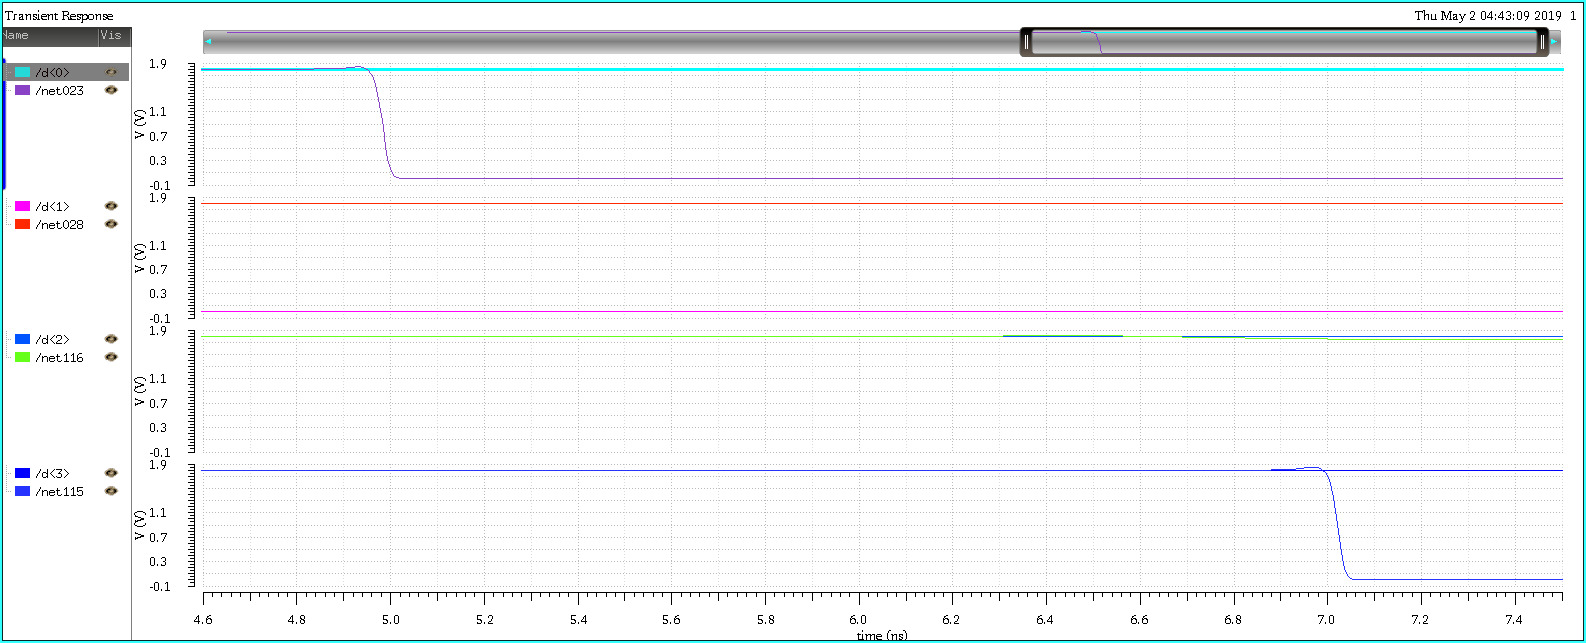
\includegraphics[width=\textwidth]{shift_left_out.jpg}
\caption{Left Shift simulation}
\end{subfigure}
\begin{subfigure}{0.7\textwidth}
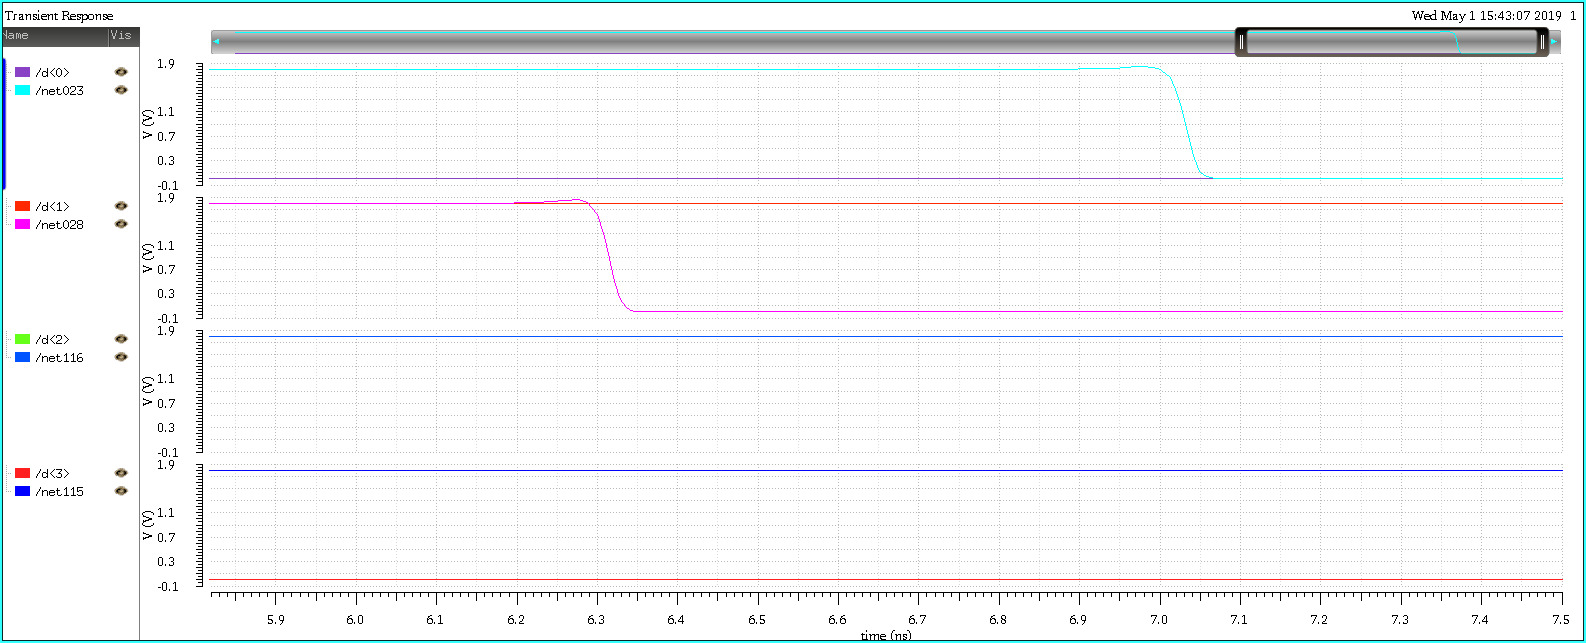
\includegraphics[width=\textwidth]{shift_out.jpg}
\caption{Right Shift simulation}
\end{subfigure}
\end{center}
\caption{Shift operation using DRAM (d is the value to be shifted)}

\end{figure}

The control signals in the shift operation are used to enable and disable many connections in the circuit, as there are connections of one output of DRAM to the input of 2 DRAMS plus to the write driver. Transmission gates are used to select signals or paths for left or right shift. Control signals will be thoroughly discussed in the further chapters.

\begin{figure}[H]
\centering
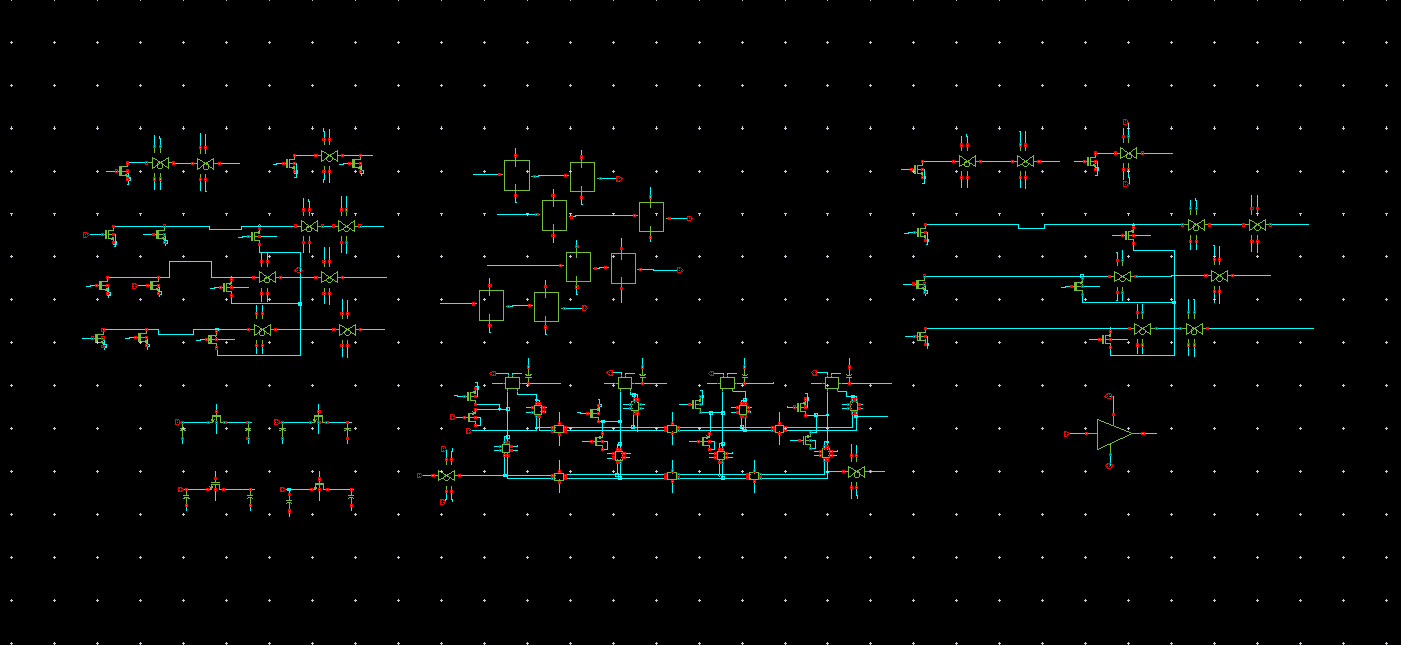
\includegraphics[width=0.7\textwidth]{shift_blk_full.png}
\caption{The complete DRAM shifter design}
\label{fig:Figure}
\end{figure}